% Options for packages loaded elsewhere
\PassOptionsToPackage{unicode}{hyperref}
\PassOptionsToPackage{hyphens}{url}
%
\documentclass[
  english,
  man]{apa6}
\title{One- vs.~Two-Step Approach in Regularized Bayesian Confirmatory Factor Analysis (CFA)}
\author{\phantom{0}}
\date{}

\usepackage{amsmath,amssymb}
\usepackage{lmodern}
\usepackage{iftex}
\ifPDFTeX
  \usepackage[T1]{fontenc}
  \usepackage[utf8]{inputenc}
  \usepackage{textcomp} % provide euro and other symbols
\else % if luatex or xetex
  \usepackage{unicode-math}
  \defaultfontfeatures{Scale=MatchLowercase}
  \defaultfontfeatures[\rmfamily]{Ligatures=TeX,Scale=1}
\fi
% Use upquote if available, for straight quotes in verbatim environments
\IfFileExists{upquote.sty}{\usepackage{upquote}}{}
\IfFileExists{microtype.sty}{% use microtype if available
  \usepackage[]{microtype}
  \UseMicrotypeSet[protrusion]{basicmath} % disable protrusion for tt fonts
}{}
\makeatletter
\@ifundefined{KOMAClassName}{% if non-KOMA class
  \IfFileExists{parskip.sty}{%
    \usepackage{parskip}
  }{% else
    \setlength{\parindent}{0pt}
    \setlength{\parskip}{6pt plus 2pt minus 1pt}}
}{% if KOMA class
  \KOMAoptions{parskip=half}}
\makeatother
\usepackage{xcolor}
\IfFileExists{xurl.sty}{\usepackage{xurl}}{} % add URL line breaks if available
\IfFileExists{bookmark.sty}{\usepackage{bookmark}}{\usepackage{hyperref}}
\hypersetup{
  pdftitle={One- vs.~Two-Step Approach in Regularized Bayesian Confirmatory Factor Analysis (CFA)},
  pdflang={en-EN},
  hidelinks,
  pdfcreator={LaTeX via pandoc}}
\urlstyle{same} % disable monospaced font for URLs
\usepackage{graphicx}
\makeatletter
\def\maxwidth{\ifdim\Gin@nat@width>\linewidth\linewidth\else\Gin@nat@width\fi}
\def\maxheight{\ifdim\Gin@nat@height>\textheight\textheight\else\Gin@nat@height\fi}
\makeatother
% Scale images if necessary, so that they will not overflow the page
% margins by default, and it is still possible to overwrite the defaults
% using explicit options in \includegraphics[width, height, ...]{}
\setkeys{Gin}{width=\maxwidth,height=\maxheight,keepaspectratio}
% Set default figure placement to htbp
\makeatletter
\def\fps@figure{htbp}
\makeatother
\setlength{\emergencystretch}{3em} % prevent overfull lines
\providecommand{\tightlist}{%
  \setlength{\itemsep}{0pt}\setlength{\parskip}{0pt}}
\setcounter{secnumdepth}{-\maxdimen} % remove section numbering
% Make \paragraph and \subparagraph free-standing
\ifx\paragraph\undefined\else
  \let\oldparagraph\paragraph
  \renewcommand{\paragraph}[1]{\oldparagraph{#1}\mbox{}}
\fi
\ifx\subparagraph\undefined\else
  \let\oldsubparagraph\subparagraph
  \renewcommand{\subparagraph}[1]{\oldsubparagraph{#1}\mbox{}}
\fi
\newlength{\cslhangindent}
\setlength{\cslhangindent}{1.5em}
\newlength{\csllabelwidth}
\setlength{\csllabelwidth}{3em}
\newlength{\cslentryspacingunit} % times entry-spacing
\setlength{\cslentryspacingunit}{\parskip}
\newenvironment{CSLReferences}[2] % #1 hanging-ident, #2 entry spacing
 {% don't indent paragraphs
  \setlength{\parindent}{0pt}
  % turn on hanging indent if param 1 is 1
  \ifodd #1
  \let\oldpar\par
  \def\par{\hangindent=\cslhangindent\oldpar}
  \fi
  % set entry spacing
  \setlength{\parskip}{#2\cslentryspacingunit}
 }%
 {}
\usepackage{calc}
\newcommand{\CSLBlock}[1]{#1\hfill\break}
\newcommand{\CSLLeftMargin}[1]{\parbox[t]{\csllabelwidth}{#1}}
\newcommand{\CSLRightInline}[1]{\parbox[t]{\linewidth - \csllabelwidth}{#1}\break}
\newcommand{\CSLIndent}[1]{\hspace{\cslhangindent}#1}
% This preamble allows to remove the redundant title page from papaja's output.pdf
\usepackage{atbegshi}% http://ctan.org/pkg/atbegshi
\AtBeginDocument{\AtBeginShipoutNext{\AtBeginShipoutDiscard}}
% Manuscript styling
\usepackage{upgreek}
\captionsetup{font=singlespacing,justification=justified}

% Table formatting
\usepackage{longtable}
\usepackage{lscape}
% \usepackage[counterclockwise]{rotating}   % Landscape page setup for large tables
\usepackage{multirow}		% Table styling
\usepackage{tabularx}		% Control Column width
\usepackage[flushleft]{threeparttable}	% Allows for three part tables with a specified notes section
\usepackage{threeparttablex}            % Lets threeparttable work with longtable

% Create new environments so endfloat can handle them
% \newenvironment{ltable}
%   {\begin{landscape}\centering\begin{threeparttable}}
%   {\end{threeparttable}\end{landscape}}
\newenvironment{lltable}{\begin{landscape}\centering\begin{ThreePartTable}}{\end{ThreePartTable}\end{landscape}}

% Enables adjusting longtable caption width to table width
% Solution found at http://golatex.de/longtable-mit-caption-so-breit-wie-die-tabelle-t15767.html
\makeatletter
\newcommand\LastLTentrywidth{1em}
\newlength\longtablewidth
\setlength{\longtablewidth}{1in}
\newcommand{\getlongtablewidth}{\begingroup \ifcsname LT@\roman{LT@tables}\endcsname \global\longtablewidth=0pt \renewcommand{\LT@entry}[2]{\global\advance\longtablewidth by ##2\relax\gdef\LastLTentrywidth{##2}}\@nameuse{LT@\roman{LT@tables}} \fi \endgroup}

% \setlength{\parindent}{0.5in}
% \setlength{\parskip}{0pt plus 0pt minus 0pt}

% \usepackage{etoolbox}
\makeatletter
\patchcmd{\HyOrg@maketitle}
  {\section{\normalfont\normalsize\abstractname}}
  {\section*{\normalfont\normalsize\abstractname}}
  {}{\typeout{Failed to patch abstract.}}
\patchcmd{\HyOrg@maketitle}
  {\section{\protect\normalfont{\@title}}}
  {\section*{\protect\normalfont{\@title}}}
  {}{\typeout{Failed to patch title.}}
\makeatother
\shorttitle{One- vs. Two-Step Approach in Regularized Bayesian CFA}
\keywords{\newline\indent Word count: X}
\DeclareDelayedFloatFlavor{ThreePartTable}{table}
\DeclareDelayedFloatFlavor{lltable}{table}
\DeclareDelayedFloatFlavor*{longtable}{table}
\makeatletter
\renewcommand{\efloat@iwrite}[1]{\immediate\expandafter\protected@write\csname efloat@post#1\endcsname{}}
\makeatother
\usepackage{csquotes}
\ifXeTeX
  % Load polyglossia as late as possible: uses bidi with RTL langages (e.g. Hebrew, Arabic)
  \usepackage{polyglossia}
  \setmainlanguage[]{english}
\else
  \usepackage[main=english]{babel}
% get rid of language-specific shorthands (see #6817):
\let\LanguageShortHands\languageshorthands
\def\languageshorthands#1{}
\fi
\ifLuaTeX
  \usepackage{selnolig}  % disable illegal ligatures
\fi


\affiliation{\phantom{0}}

\begin{document}
\maketitle

% move text to bottom of page
\vfill
Research Proposal \\
Michael Koch (6412157)\\
Methodology and Statistics for the Behavioral, Biomedical, and Social Sciences \\
Supervisor: Dr. Sara van Erp \\ 
Email: j.m.b.koch@students.uu.nl \\
Word Count: 817 \\
Intented Journal of Publication: Structural Equation Modeling \\
FETC permission obtained on 27'th September 2021

% make page numbers start from second page 
\pagenumbering{arabic}
\setcounter{page}{0}
\thispagestyle{empty}
% make page numbers from second page 
\pagestyle{plain}

\clearpage

A common model-constraint in \emph{Confirmatory Factor Analysis (CFA)} is fixing all cross-loadings to zero. This is done both to identify the model, and to achieve an easy-to-interpret factor structure. However, this practice often leads to poor model fit. Consequently, researchers commonly free some cross-loadings based on modification indices to improve model fit. This practice, however, is flawed for a variety of reasons, among which risking capitalization on chance (Jacobucci, Grimm, \& McArdle, 2016; Muthen \& Asparouhov, 2012).

As solution, Muthen and Asparouhov (2012) proposed that rather than fixing all cross-loadings to zero, one should should assume that \emph{most} cross-loadings are zero. Formally, this is achieved by setting the so called \emph{Small Variance Prior} for the cross-loadings, which is a normal distribution with mean zero and a very small variance (e.g.: \(\sigma = 0.01, \  \sigma = 0.001\)). Such prior gives cross-loadings of zero large prior density, but cross-loadings that are far from zero almost zero prior density (see Figure 1 for an example with \(\sigma = 0.01\)). Consequently, all cross-loadings in the model are shrunken substantially, those close to zero to zero, and those far from zero towards zero. The prior's variance is thus the deciding factor in how admissive the model is of cross-loadings closer to zero. Hence, by tuning the variance of the prior, one is able to fit a systematically and continuously varying sequence of models allowing for a much more continuous process of model identification and model selection than classical CFA.

However, an issue with this method is that not only the cross-loadings close to zero that are considered irrelevant are shrunken to zero, as desired. Also the cross-loadings that are further from zero, are shrunken towards zero, which introduces bias. The method thus requires a two-step approach. First, the model is estimated with shrinkage. Then the model is re-estimated where the cross-loadings that have been shrunken to zero in the previous step are fixed to zero, and the remaining cross-loadings are estimated without shrinkage. To overcome this, alternative regularization priors need to be identified that can outperform the small-variance prior \emph{in a single step}.

Lu, Chow, and Loken (2016) pointed out that the Bayesian CFA approach by Muthen and Asparouhov (2012) can be viewed as a form of \emph{Regularization}, where rather than selecting variables that are relevant as predictors in a regression model, cross-loadings that are relevant in modeling a factor structure are selected. The literature on regularization in a regression context (see Van Erp, Oberski, \& Mulder, 2019 for an overview) can thus provide alternative priors. Here, the \emph{Regularized Horseshoe Prior} (Piironen \& Vehtari, 2017), an extension of the \emph{Horseshoe prior} (Carvalho, Polson, \& Scott, 2010), appears as particularly promising. Both priors are characterized by a \emph{global} shrinkage component \(\omega\), shrinking all parameters towards zero (explaining the steep peak \(\lambda_c = 0\) in Figure 1), and a \emph{local} component \(\tau_j\), which gives the prior its heavy tails and thereby allows large parameters to escape the shrinkage entirely\footnote{We deviate from the common notation of the global shrinkage parameter as \(\lambda\), as that letter is commonly reserved for factor loadings in CFA.}. Although being one of the core qualities of the original Horseshoe Prior, in practice not shrinking large coefficients at all can lead to computational issues in the MCMC sampling of the model (Ghosh, Li, \& Mitra, 2018; Piironen \& Vehtari, 2017). To avoid this, the \emph{Regularized} Horseshoe Prior\footnote{Following previous research, we set the hyper-parameters \(\nu = 4\) and \(s^2 = 2\) (Piironen \& Vehtari, 2017; Van Erp et al., 2019).} is designed to ensure that there is always a little shrinkage, even for large parameters (Piironen \& Vehtari, 2017):

\[\lambda_c | \hat{\tau}, \omega \sim \mathcal{N}(0, \ \hat{\tau}^2 \omega), \ with \ \hat{\tau}^2 = \frac{c^2\tau_j^2}{c^2 + \omega^2 \tau_j^2}\]
\[\omega | \omega_0^2 \sim \mathcal{N}(0,\  \omega_0^2), \ with \  \omega_0 = \frac{p_0}{p-p_0}\frac{\sigma}{\sqrt{N}}\]
\[\tau_j \sim \mathcal{C^+}(0, \ 1)\]
\[c^2 | \nu, s^2 \sim \mathcal{IG}(\nu/2, \  \nu s^2/2),\]
where \(p_0\) represents a prior guess of the number of relevant cross-loadings.

\begin{figure}
\centering
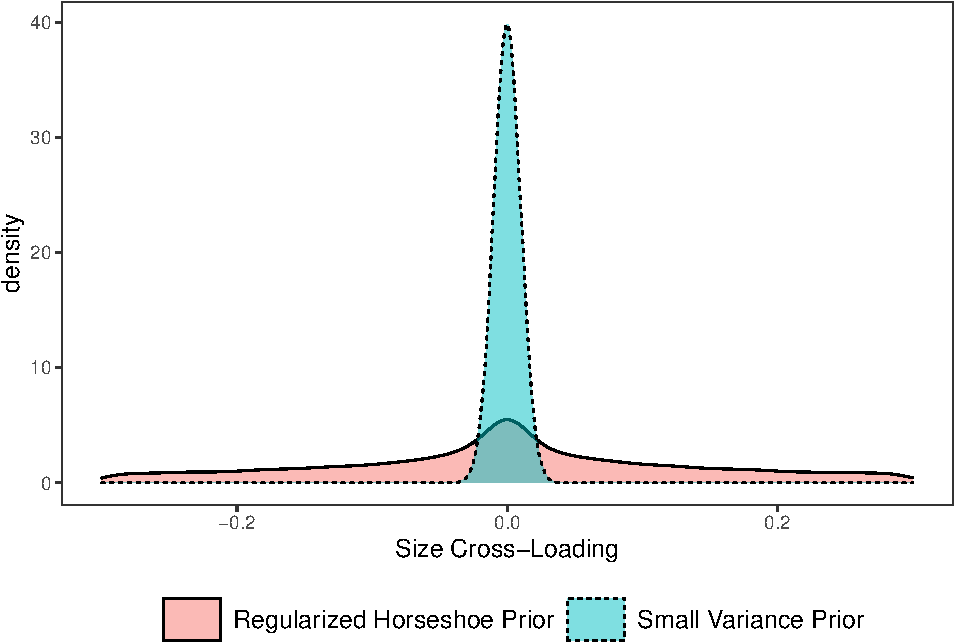
\includegraphics{JMBKoch_Proposal_files/figure-latex/unnamed-chunk-1-1.pdf}
\caption{\label{fig:unnamed-chunk-1}Density Plots of the Regularization Priors of Interest}
\end{figure}

While the Regularized Horseshoe Prior has been shown to perform well in the selection of relevant predictors in regression (Piironen \& Vehtari, 2017; Van Erp et al., 2019), no previous research has validated its performance in the context of selecting relevant cross-loadings in CFA. To fill this gap, the aim of this study is to compare the Regularized Horseshoe Prior to the Small Variance Prior in their performance in selecting the true factor structure in Confirmatory Factor Analysis (CFA).

\hypertarget{analytic-strategy}{%
\subsection{Analytic Strategy}\label{analytic-strategy}}

A Monte Carlo simulation study is conducted using stan (Carpenter et al., 2017).
True Positives vs.~False Positives in estimating truly non-zero cross-loadings as non-zero are considered as main outcome.
Conditions are based on (Lu et al., 2016) and will include two factor structures (1 non-zero cross-loading, several non-zero cross-loadings), three sample sizes (100, 200, 300), and three magnitudes of the cross-loadings (0.1, 0.2, 0.3), yielding a total of \(2 \times 3 \times 3 = 18\) main conditions. All models will be sampled using the NUTS-sampler (Betancourt, 2018), where each time four chains are sampled for 1000 iterations, following a burn-in-period of 1000.

\clearpage

\hypertarget{references}{%
\section{References}\label{references}}

\begingroup
\setlength{\parindent}{-0.5in}
\setlength{\leftskip}{0.5in}

\hypertarget{refs}{}
\begin{CSLReferences}{1}{0}
\leavevmode\vadjust pre{\hypertarget{ref-betancourt_conceptual_2018}{}}%
Betancourt, M. (2018). A {Conceptual} {Introduction} to {Hamiltonian} {Monte} {Carlo}. \emph{arXiv:1701.02434 {[}Stat{]}}. Retrieved from \url{http://arxiv.org/abs/1701.02434}

\leavevmode\vadjust pre{\hypertarget{ref-carpenter_stan_2017}{}}%
Carpenter, B., Gelman, A., Hoffman, M. D., Lee, D., Goodrich, B., Betancourt, M., \ldots{} Riddell, A. (2017). Stan: {A} {Probabilistic} {Programming} {Language}. \emph{Journal of Statistical Software}, \emph{76}(1), 1--32. \url{https://doi.org/10.18637/jss.v076.i01}

\leavevmode\vadjust pre{\hypertarget{ref-carvalho_horseshoe_2010}{}}%
Carvalho, C. M., Polson, N. G., \& Scott, J. G. (2010). The horseshoe estimator for sparse signals. \emph{Biometrika}, \emph{97}(2), 465--480. \url{https://doi.org/10.1093/biomet/asq017}

\leavevmode\vadjust pre{\hypertarget{ref-ghosh_use_2018}{}}%
Ghosh, J., Li, Y., \& Mitra, R. (2018). On the {Use} of {Cauchy} {Prior} {Distributions} for {Bayesian} {Logistic} {Regression}. \emph{Bayesian Analysis}, \emph{13}(2), 359--383. \url{https://doi.org/10.1214/17-BA1051}

\leavevmode\vadjust pre{\hypertarget{ref-jacobucci_regularized_2016}{}}%
Jacobucci, R., Grimm, K. J., \& McArdle, J. J. (2016). Regularized {Structural} {Equation} {Modeling}. \emph{Structural Equation Modeling: A Multidisciplinary Journal}, \emph{23}(4), 555--566. \url{https://doi.org/10.1080/10705511.2016.1154793}

\leavevmode\vadjust pre{\hypertarget{ref-lu_bayesian_2016}{}}%
Lu, Z.-H., Chow, S.-M., \& Loken, E. (2016). Bayesian {Factor} {Analysis} as a {Variable}-{Selection} {Problem}: {Alternative} {Priors} and {Consequences}. \emph{Multivariate Behavioral Research}, \emph{51}(4), 519--539. \url{https://doi.org/10.1080/00273171.2016.1168279}

\leavevmode\vadjust pre{\hypertarget{ref-muthen_bayesian_2012}{}}%
Muthen, B., \& Asparouhov, T. (2012). Bayesian {SEM}: {A} more flexible representation of substantive theory, 78. \url{https://doi.org/10.1037/a0026802}

\leavevmode\vadjust pre{\hypertarget{ref-piironen_sparsity_2017}{}}%
Piironen, J., \& Vehtari, A. (2017). Sparsity information and regularization in the horseshoe and other shrinkage priors. \emph{Electronic Journal of Statistics}, \emph{11}(2), 5018--5051. \url{https://doi.org/10.1214/17-EJS1337SI}

\leavevmode\vadjust pre{\hypertarget{ref-van_erp_shrinkage_2019}{}}%
Van Erp, S., Oberski, D. L., \& Mulder, J. (2019). Shrinkage priors for {Bayesian} penalized regression. \emph{Journal of Mathematical Psychology}, \emph{89}, 31--50. \url{https://doi.org/10.1016/j.jmp.2018.12.004}

\end{CSLReferences}

\endgroup


\end{document}
